\documentclass[oneside]{article}

% Language setting
% Replace `english' with e.g. `spanish' to change the document language
\usepackage[english]{babel}
\usepackage[utf8]{inputenc} % für Umlaute
\usepackage{fontenc}

% Set page size and margins
% Replace `letterpaper' with`a4paper' for UK/EU standard size
\usepackage[a4paper,top=2cm,bottom=2cm,left=3cm,right=3cm,marginparwidth=1.75cm]{geometry}

%%%% ---- Useful packages

%%% --- Figures and Graphics
\usepackage{graphicx}
\usepackage{subcaption}
\usepackage{tikz}

%%% --- Colors
\usepackage[]{xcolor}

%%% --- Tabulars
\usepackage{booktabs}
\usepackage{multirow} % cells over several rows
\usepackage{tabularx}

%%% --- Mathematics
\usepackage{amsmath,amsfonts,amssymb,amsthm,mathtools, mathabx}
\usepackage{bm} % bold mathematics
\usepackage{bbm} % for blackboard 1
\usepackage[linesnumbered,lined,algo2e,figure,boxed]{algorithm2e}
\usepackage[short]{optidef} % for aligning linear programs

%%% --- Other
\usepackage[colorlinks=true, allcolors=blue]{hyperref}
%\usepackage[hidelinks]{hyperref}
\usepackage[style=authoryear,backend=bibtex]{biblatex}
%\addbibresource{library.bib}
\usepackage{csquotes}
\usepackage[shortcuts]{extdash} % For Hyphens in English
%\usepackage{acro}
% \DeclareAcronym{pdf}{short=PDF, long={probability distribution function}}

%%% --- Commenting, Todonotes
\usepackage[colorinlistoftodos,prependcaption,textsize=tiny]{todonotes}
\usepackage{comment, soul}
\newcommand{\ar}{$\rightarrow$}
\presetkeys{todonotes}{backgroundcolor=yellow!30, bordercolor=yellow!50, linecolor=yellow!50, figwidth=\textwidth}{}
%\newcommand{\hl}[1]{\textcolor{Aquamarine}{#1}}

\usepackage{xargs} % Use optional arguements in commands
\newcommandx{\unsure}[2][1=]{\todo[linecolor=blue,backgroundcolor=blue!25,bordercolor=blue,#1]{#2}}
\newcommandx{\missing}[2][1=]{\todo[linecolor=red,backgroundcolor=red!25,bordercolor=red,#1]{#2}}
\newcommandx{\change}[2][1=]{\todo[linecolor=red,backgroundcolor=red!25,bordercolor=red,#1]{#2}}
\newcommandx{\info}[2][1=]{\todo[linecolor=OliveGreen,backgroundcolor=OliveGreen!25,bordercolor=OliveGreen,#1]{#2}}
\newcommandx{\improvement}[2][1=]{\todo[linecolor=Plum,backgroundcolor=Plum!25,bordercolor=Plum,#1]{#2}}
\newcommandx{\thiswillnotshow}[2][1=]{\todo[disable,#1]{#2}}
\usepackage{marginnote}
\let\marginpar\marginnote

%%%% ---- Own Commands
%%% --- Theorem Settings
\theoremstyle{plain}% Theorem-like structures provided by amsthm.sty
\newtheorem{theorem}{Theorem}
\newtheorem{exa}{Example}
\newtheorem{rem}{Remark}
\newtheorem{proposition}{Proposition}
\newtheorem{lemma}{Lemma}
\newtheorem{corollary}{Corollary}

\theoremstyle{definition}
\newtheorem{definition}{Definition}
\newtheorem{remark}{Remark}
\newtheorem{example}{Example}

%%% --- Math Commands

\newcommand{\lag}[1][l]{\Delta_{#1}}
\DeclarePairedDelimiter{\abs}\lvert\rvert
\DeclareMathOperator{\sign}{sign}
\newcommand{\tmax}{\bar{t}}
\newcommand{\ind}[1]{\mathbbm{1}\{#1\}}
\newcommand{\ydiff}{\overset{\smalltriangleup}{y}}
\newcommand{\ydifft}{\overset{\smalltriangleup}{y}^*}
\newcommand{\xdiff}{\overset{\smalltriangleup}{x}}
\newcommand{\xdifft}{\overset{\smalltriangleup}{x}^*}
\newcommand{\Ydiff}{\overset{\smalltriangleup}{Y}}
\newcommand{\Xdiff}{\overset{\smalltriangleup}{X}}
\newcommand{\Prob}[1]{P(#1)}
\newcommand{\mprob}{\tilde{m}}
\newcommand{\Ber}{\text{Ber}}
\newcommand{\SBer}{\text{SBer}}

%%% --- Other Commands
\renewcommand{\arraystretch}{1.2}

%%% --- ToDo List
\usepackage{enumitem}
\newlist{todolist}{itemize}{2}
\setlist[todolist]{label=$\square$}
\usepackage{pifont}
\newcommand{\cmark}{\ding{51}}%
\newcommand{\xmark}{\ding{55}}%
\newcommand{\done}{\rlap{$\square$}{\raisebox{2pt}{\large\hspace{1pt}\cmark}}%
\hspace{-2.5pt}}
\newcommand{\wontfix}{\rlap{$\square$}{\large\hspace{1pt}\xmark}}

\title{Assessment and Optimization of Nowcast Measures for Trend Detection}
\author{Oliver Grothe, Bolin Liu, Jonas Rieger}

\begin{document}
\maketitle

\begin{abstract}
Existing and new measures for the capability of capturing the trend of nowcasts are presented, evaluated, and compared on synthetic and real-world data.
\end{abstract}

\subsection*{Offene Punkte}

\begin{itemize}
    \item was ist mit dem Trendinghorizont, also welche Zeitinkremente sind zu nehmen. Da würde sich irgendwie ein Plot Maß gegen Inkrement anbieten. Dann würden sich für unterschiedliche Inkremente unterschiedliche Trendingcapabilities ergeben (gabe es nicht so einen schonmal bei irgendeinem Treffen?)
    \item Wahl des Rauschens; haben wir da irgendeine Methode aus den Daten das Sigma zu bekommen?
    \item Was ist mit anderen Verteilungen?
    \item Nicht nur Nowcast, sondern auch Measurement und Forecasts; in Introduction Unterschiede zwischen den Feldern; mehr Literatur; Einleitung ausbauen
\end{itemize}

\listoftodos

Für nächstes Treffen:
\begin{itemize}
    \item Wie wird $\sigma$ geschätzt? Literaturrecherche, wo sonst noch \enquote{beliebig} festgelegt wird?
\end{itemize}

\section{Introduction}

\begin{itemize}
	\item Trending is an important feature of nowcasts to be identify changes in the situation before the actual quantity can be measured
	\item What scores are currently used?
	\item Examples: Covid, BIP, Medicine, ... 
\end{itemize}


\section{Trend measures for nowcasts}

Notation
\begin{itemize}
  \item Let $y_1, \ldots, y_T$ be the values of the nowcasted quantity.
  \item Let $x_t^k$ be the $k$-th nowcast for time $t = 1, \ldots, T$ (possibly after some aggregation if several raw nowcasts apply).
  \item Let $\ydiff_t = y_t - y_{t-1}$ be the change that occurred between the time steps $t-1$ and $t$ and $\xdiff_t^k = x_t - y_{t-1}$ the change nowcaster $k$ issued between the time steps. 
  \item Then, $\xdiff_t^k$ can be seen as point forecast of $\ydiff_t$. 
\end{itemize}

\todo[inline]{$\xdiff_t^k = x_t - y_{t-1}$ oder $x_{t-1}$? Evtl. mit Bezug zu Verzögerung des Bekanntwerdens von $y_{t-1}$.}

\subsection{What is the trend of a nowcast?}

Trend: Issuing the right \enquote{direction} of change between two time steps

\begin{itemize}
  \item Translate into mathematical notation
  \item Illustrative Example: Two nowcasts of quantity of interest, where one jumps up and down and one points in right direction with the same rmse; small subset of Simulation~\ref{sec:simulation_rmse_mae}; Plot time series \& time series of differences
\end{itemize}

\subsection{Graphical methods}

Bolin

\begin{itemize}
  \item 4Q-Plot
  \item Andere Medizin-Plots mit Verweis auf Grothe-Paper
\end{itemize}


\subsection{Measures}

%\begin{table}
%	\centering
%	\begin{tabular}{l l c c}
%	\toprule
%	& & \multicolumn{2}{c}{Observed trend} \\
%	& & $\ydiff_t > 0$ & $\ydiff_t < 0$ \\	\cline{3-4}
%	\multirow{2}{*}{Forecasted trend} & $\xdiff_t > 0$ & hit & false alarm\\
%	& $\xdiff_t < 0$ & miss & correct negative \\
%	\bottomrule
%\end{tabular}
%\end{table}

Non-probabilistic measures: Summation anpassen; sodass rolling windows einfacher; untere Summationsgrenze $T - l$ ($l$ rolling window Größe); Nochmal anschauen, was unbeobachtbar und was beobachtbar ist; "verrauschtes" echtes kann auch daher kommen, dass ich nicht unbedingt $x - y_{t-1}$ rechnen kann

\begin{itemize}
  \item Accuracy: \begin{equation}
  	m_{\text{acc}} = \frac{\sum_{t=2}^T \ind{\ydiff_t > 0, \xdiff_t > 0} + \sum_{t=2}^T \ind{\ydiff_t < 0, \xdiff_t < 0}}{T-1}
\end{equation}
	\item Capability of detecting a positive trend (probability of detection)
	\begin{equation}
  		m_{\text{py}} = \frac{\sum_{t=2}^T \ind{\ydiff_t > 0, \xdiff_t > 0}}{\sum_{t=2}^T \ind{\ydiff_t > 0}}
	\end{equation}
	\item False alarm rate \hl{Name does not fit} \begin{equation}
  m_{\text{far}} = \frac{\sum_{t=2}^T \ind{\ydiff_t < 0, \xdiff_t > 0}}{\sum_{t=2}^T \ind{\xdiff_t > 0}}
\end{equation}
maybe use \enquote{positive} measure instead, i.e.,
\begin{equation}
  m_{\text{px}} = \frac{\sum_{t=2}^T \ind{\ydiff_t > 0, \xdiff_t > 0}}{\sum_{t=2}^T \ind{\xdiff_t > 0}}  
\end{equation}
	\item same measures for negative direction:
	\begin{align}
		m_{\text{ny}} &=  \frac{\sum_{t=2}^T \ind{\ydiff_t < 0, \xdiff_t < 0}}{\sum_{t=2}^T \ind{\ydiff_t < 0}} \\
		m_{\text{nx}} &=  \frac{\sum_{t=2}^T \ind{\ydiff_t < 0, \xdiff_t < 0}}{\sum_{t=2}^T \ind{\xdiff_t < 0}}
	\end{align}
\end{itemize}

Resulting measures:
\begin{itemize}
  % \item Scoring rules for probabilities

% \begin{itemize}
%   \item Quadratic/Brier Score for $k$ possible outcomes \hl{Erst mal rauslassen; wäre anderes setting: probabilistischer Nowcast}: \begin{equation}
%   S((p_1, \dots, p_k), i) = 2 p_i - \sum_{l=1}^k p_i^2 - 1;
% \end{equation}
% for dichotomous outcomes ($p_1 = \hat{P}(\ydiff_t > 0)$: probability for $\ydiff_t > 0$):
% \begin{equation}
%   S(p_1, \ydiff_t) = p_1 \ind{\ydiff_t > 0} + (1 - p_1) (1 - \ind{\ydiff_t > 0}) + p_1^2 + (1-p_1)^2 - 1
% \end{equation}
% \end{itemize}
\item Probabilistic versions of non-probabilistic measures:
\begin{itemize}
  \item Assume an additive error decomposition for both observation and nowcast to account for non-systematic and short-term (i.e., intra-day) effects:
  	\begin{align}
  		\ydiff_t &= \ydifft + \varepsilon_t^y \\
  		\xdiff_t &= \xdifft + \varepsilon_t^x
	\end{align}
\item  Replace indicators in the above formulations by the corresponding probabilities:
\begin{align}
		\mprob_{\text{acc}} &= \frac{\sum_{t=2}^T \Prob{ \ydifft_t > 0, \xdifft_t > 0} + \sum_{t=2}^T \Prob{\ydifft_t < 0, \xdifft_t < 0}}{T-1}  \\
   \mprob_{\text{py}} &= \frac{\sum_{t=2}^T \Prob{\ydifft_t > 0, \xdifft_t > 0}}{\sum_{t=2}^T \Prob{\ydifft_t > 0}} \\
    \mprob_{\text{px}} &= \frac{\sum_{t=2}^T \Prob{\ydifft_t > 0, \xdifft_t > 0}}{\sum_{t=2}^T \Prob{\xdifft_t > 0}} \\
    \mprob_{\text{ny}} &= \frac{\sum_{t=2}^T \Prob{\ydifft_t < 0, \xdifft_t < 0}}{\sum_{t=2}^T \Prob{\ydifft_t < 0}} \\
    \mprob_{\text{px}} &= \frac{\sum_{t=2}^T \Prob{\ydifft_t < 0, \xdifft_t < 0}}{\sum_{t=2}^T \Prob{\xdifft_t < 0}} 
\end{align}
\item Simple error model:
  \begin{align}
	  \varepsilon_Y \sim N(0, \sigma_Y) \\
	  \varepsilon_X \sim N(0, \sigma_X)
  \end{align}
  yields, e.g.,
  	\begin{equation}
  		\mprob_{\text{acc}} = \frac{\sum_{t=2}^T  \big( 1 - \Phi_{\ydiff_t, \sigma_y}(0) - \Phi_{\xdiff_t, \sigma_x} (0) + 2 \Phi_{(\ydiff_t, \xdiff_t); (\sigma_y, \sigma_x)}( 0, 0) \big) }{T-1}, 
	\end{equation}
	where $\Phi$ denotes a (possibly multivariate) normal distribution
\end{itemize}
\end{itemize}

\todo[inline]{Annahmen an $\varepsilon$: white noise; wie kommt man auf den Wert? Ideen: Expertenwissen, Anteil an Gesamtvarianz der Zeitreihen (z.B. 10 \%), \textbf{Literaturrecherche zu wie das sonst so gemacht werden könnte}}

\subsection{Confidence intervals and missing data}

Bolin

\begin{itemize}
  \item Bootstrapping: Compare percentile and BCa approach?
  \item Bootstrapping: What is the \enquote{true} value?
  \item Missing data
\end{itemize}


\section{Simulation studies}

\subsection{Different trending abilities for same rmse and mae} \label{sec:simulation_rmse_mae}

Let the quantity of interest 
\begin{equation}
  y_t = a \sin(2 \pi t / T) + \varepsilon_t^y, \ t = 1, \dots, T
\end{equation}
with $\varepsilon_t^y \stackrel{\text{iid}}{\sim} N(0, \sigma_y)$ and 
\begin{equation}
  \ydiff_t = y_t - y_{t-1}.
\end{equation}
The nowcasts are characterised by 
\begin{align}
	\xdiff_t^1 &= e^x_t \ydiff_t \\
	\xdiff_t^2 &= \begin{cases}
		e^x_t \ydiff_t &, \text{if}\ q^2_t = 0 \lor e^x_t > 0\\
		(| e^x_t | + 2) \ydiff_t &, \text{if}\ q^2_t = 1 \land e^x_t < 0
	\end{cases} \\
	\xdiff_t^3 &= \begin{cases}
		e^x_t \ydiff_t &, \text{if}\ (q^{3, \text{down}}_t = 0 \lor e^x_t > 0) \land \ydiff_t \geq 0\\
		(| e^x_t | + 2) \ydiff_t &, \text{if}\ (q^{3, \text{down}}_t = 1 \land e^x_t < 0) \land \ydiff_t \geq 0 \\
		e^x_t \ydiff_t &, \text{if}\ (q^{3, \text{up}}_t = 0 \lor e^x_t > 0) \land \ydiff_t < 0\\
		(| e^x_t | + 2) \ydiff_t &, \text{if}\ (q^{3, \text{up}}_t = 1 \land e^x_t < 0) \land \ydiff_t < 0
	\end{cases}
\end{align}
where $q^2_t \sim \text{Ber}(p_2)$ and $p_2$ denotes the probability that the direction of nowcast 2 is corrected and for nowcast 3 with $q^{3, \text{up}}_t \sim \text{Ber}(p_3^{\text{up}})$, $q^{3, \text{down}}_t \sim \text{Ber}(p_3^{\text{down}})$ the probabilities of direction correction depend on the direction of change. $e^x_t \sim N(0, 1)$

\begin{figure}
  \centering
  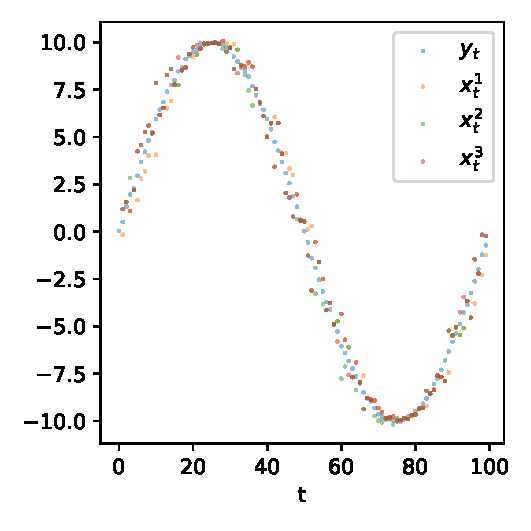
\includegraphics{plots/simulation_same_rmse_mae/time_series.pdf}
  \caption{Realisation of Simulation~\ref{sec:simulation_rmse_mae} with $T = 100$, $\sigma_y=0.1$, $a = 10$, $p_2 = 0.8$, and $p_3 = (0.8, 0.4)$}
  \label{fig:simulation_rmse_mae_ts}
\end{figure}

\begin{figure}
  \centering
  \begin{subfigure}{.32\textwidth}
  	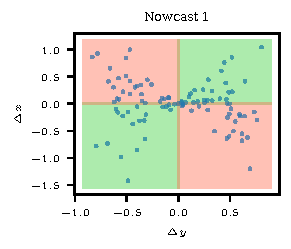
\includegraphics{plots/simulation_same_rmse_mae/4q_plot_1}
  \end{subfigure}
  \begin{subfigure}{.32\textwidth}
  	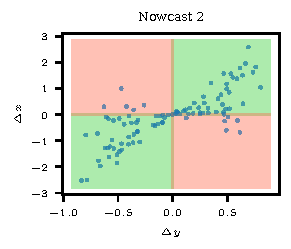
\includegraphics{plots/simulation_same_rmse_mae/4q_plot_2}
  \end{subfigure}
    \begin{subfigure}{.32\textwidth}
  	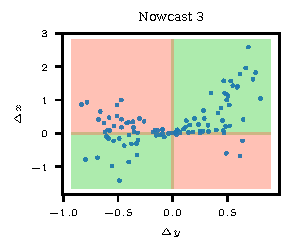
\includegraphics{plots/simulation_same_rmse_mae/4q_plot_3}
  \end{subfigure}
  \caption{4Q-Plot for Simulation~\ref{sec:simulation_rmse_mae} with $T = 100$, $\sigma_y=0.1$, $a = 10$, $p_2 = 0.8$, and $p_3 = (0.8, 0.4)$.}
  \label{fig:simulation_rmse_mae_4q}
\end{figure}

\todo[inline]{Add results}

\subsection{Simulation: Bootstrap}

Simulation setup:

\begin{itemize}
  \item $T = 10,000$
  \item $\ydiff_t \sim N(0, 1)$ 
  \item $\xdiff_t^{1, k} = b_t  \ydiff_t, b_t \sim \SBer(k)$ (symmetric Bernoulli)
\end{itemize}
\unsure[inline]{(or both + random (non-systematic) noise?)}

Analysis:
\begin{itemize}
\item Do for $l = 1, \dots, 100$:
\begin{itemize}
  \item Sample $\ydiff, \xdiff$
  \item Compute bootstrap confidence intervals $(b_{low}, b_{up})_l$ using $B = 10,000$
\end{itemize}
  \item Visualize all intervals with real value (confidence interval should cover real value in $\alpha$ cases)
\end{itemize}



\subsection{Effect of increasing sample size?}

\section{Application on disease and economic data}

\subsection{Nowcasts for the COVID infections in Germany}

\begin{itemize}
  \item Describe QoI and Nowcasts; which nowcasts do we consider? Which data is available when?
  \item Plot data
\end{itemize}

\subsection{Nowcasting of GDP}

\section{Conclusion}

\end{document} 